%% LyX 1.3 created this file.  For more info, see http://www.lyx.org/.
%% Do not edit unless you really know what you are doing.
\documentclass[english, 12pt]{article}
\usepackage{times}
%\usepackage{algorithm2e}
\usepackage{url}
\usepackage{bbm}
\usepackage[T1]{fontenc}
\usepackage[latin1]{inputenc}
\usepackage{geometry}
\geometry{verbose,letterpaper,tmargin=2cm,bmargin=2cm,lmargin=1.5cm,rmargin=1.5cm}
\usepackage{rotating}
\usepackage{color}
\usepackage{graphicx}
\usepackage{amsmath, amsthm, amssymb}
\usepackage{setspace}
\usepackage{lineno}
\usepackage{hyperref}
\usepackage{bbm}
\usepackage{makecell}
\usepackage{placeins}
\usepackage{subcaption}

%\renewcommand{\arraystretch}{1.8}

%\linenumbers
%\doublespacing
\onehalfspacing
%\usepackage[authoryear]{natbib}
\usepackage{natbib} \bibpunct{(}{)}{;}{author-year}{}{,}

%Pour les rajouts
\usepackage{color}
\definecolor{trustcolor}{rgb}{0,0,1}

\usepackage{dsfont}
\usepackage[warn]{textcomp}
\usepackage{adjustbox}
\usepackage{multirow}
\usepackage{subcaption}
\usepackage{graphicx}
\graphicspath{{../figures/}}
\DeclareMathOperator*{\argmin}{\arg\!\min}

\let\tabbeg\tabular
\let\tabend\endtabular
\renewenvironment{tabular}{\begin{adjustbox}{max width=0.95\textwidth}\tabbeg}{\tabend\end{adjustbox}}

\makeatletter

%%%%%%%%%%%%%%%%%%%%%%%%%%%%%% LyX specific LaTeX commands.
%% Bold symbol macro for standard LaTeX users
%\newcommand{\boldsymbol}[1]{\mbox{\boldmath $#1$}}

%% Because html converters don't know tabularnewline
\providecommand{\tabularnewline}{\\}
\renewcommand*{\arraystretch}{1.2}

\usepackage{babel}
\makeatother


\begin{document}

\renewcommand{\thefigure}{S\arabic{figure}}
\setcounter{figure}{0}
\renewcommand{\thetable}{S\arabic{table}}
\setcounter{table}{0}
\renewcommand{\theequation}{S\arabic{equation}}
\setcounter{equation}{0}

\section*{Supplementary Tables and Figures}

\vspace{5em}

%%%%%%%%%%%%%%%%%%%%%%%%%%%%%%%%%%%%%%%%%%%%%%%%%%%%%%%%%%%%%%%%%%%%%%%%%%%%%%%%

\begin{figure}[htbp]
	\centerline{\includegraphics[width=0.9\textwidth]{ratio-dist}}
	\caption{Relative predictive performance with UK compared to the PC distance with UK between centers of ancestry groups \cite[]{prive2020ancestry}. Relative performance values are the ones reported in Figure 1 of the main text.}
	\label{fig:ratio-dist}
\end{figure}

\begin{figure}[h]
	\centering
	\includegraphics[width=0.9\textwidth]{lasso-ancestry-geno}
	\caption{Partial correlation (and 95\% CI) in the UK test set and a test set from another ancestry group. Each point represents a phenotype (only 83 of the continuous phenotypes here) and training has been performed with penalized regression on UK individuals (training 1 in table 1) and \textbf{genotyped} variants. The slope (in blue) is computed using Deming regression with the CIs as standard deviations.
	This slope (squared) is provided in the title, which we report as the relative predictive performance compared to testing in UK.}
	\label{fig:lasso-ancestry-geno}
\end{figure}

\begin{figure}[h]
\centering
\includegraphics[width=0.9\textwidth]{ldpred2-ancestry}
\caption{Partial correlation (and 95\% CI) in the UK test set and a test set from another ancestry group. Each point represents a phenotype and training has been performed with \textbf{LDpred2-auto} on UK individuals (training 1 in table 1) and HapMap3 variants. The slope (in blue) is computed using Deming regression with the CIs as standard deviations.
This slope (squared) is provided in the title, which we report as the relative predictive performance compared to testing in UK.}
\label{fig:ldpred2-ancestry}
\end{figure}

%%%%%%%%%%%%%%%%%%%%%%%%%%%%%%%%%%%%%%%%%%%%%%%%%%%%%%%%%%%%%%%%%%%%%%%%%%%%%%%%

\begin{figure}[h]
	\centering
	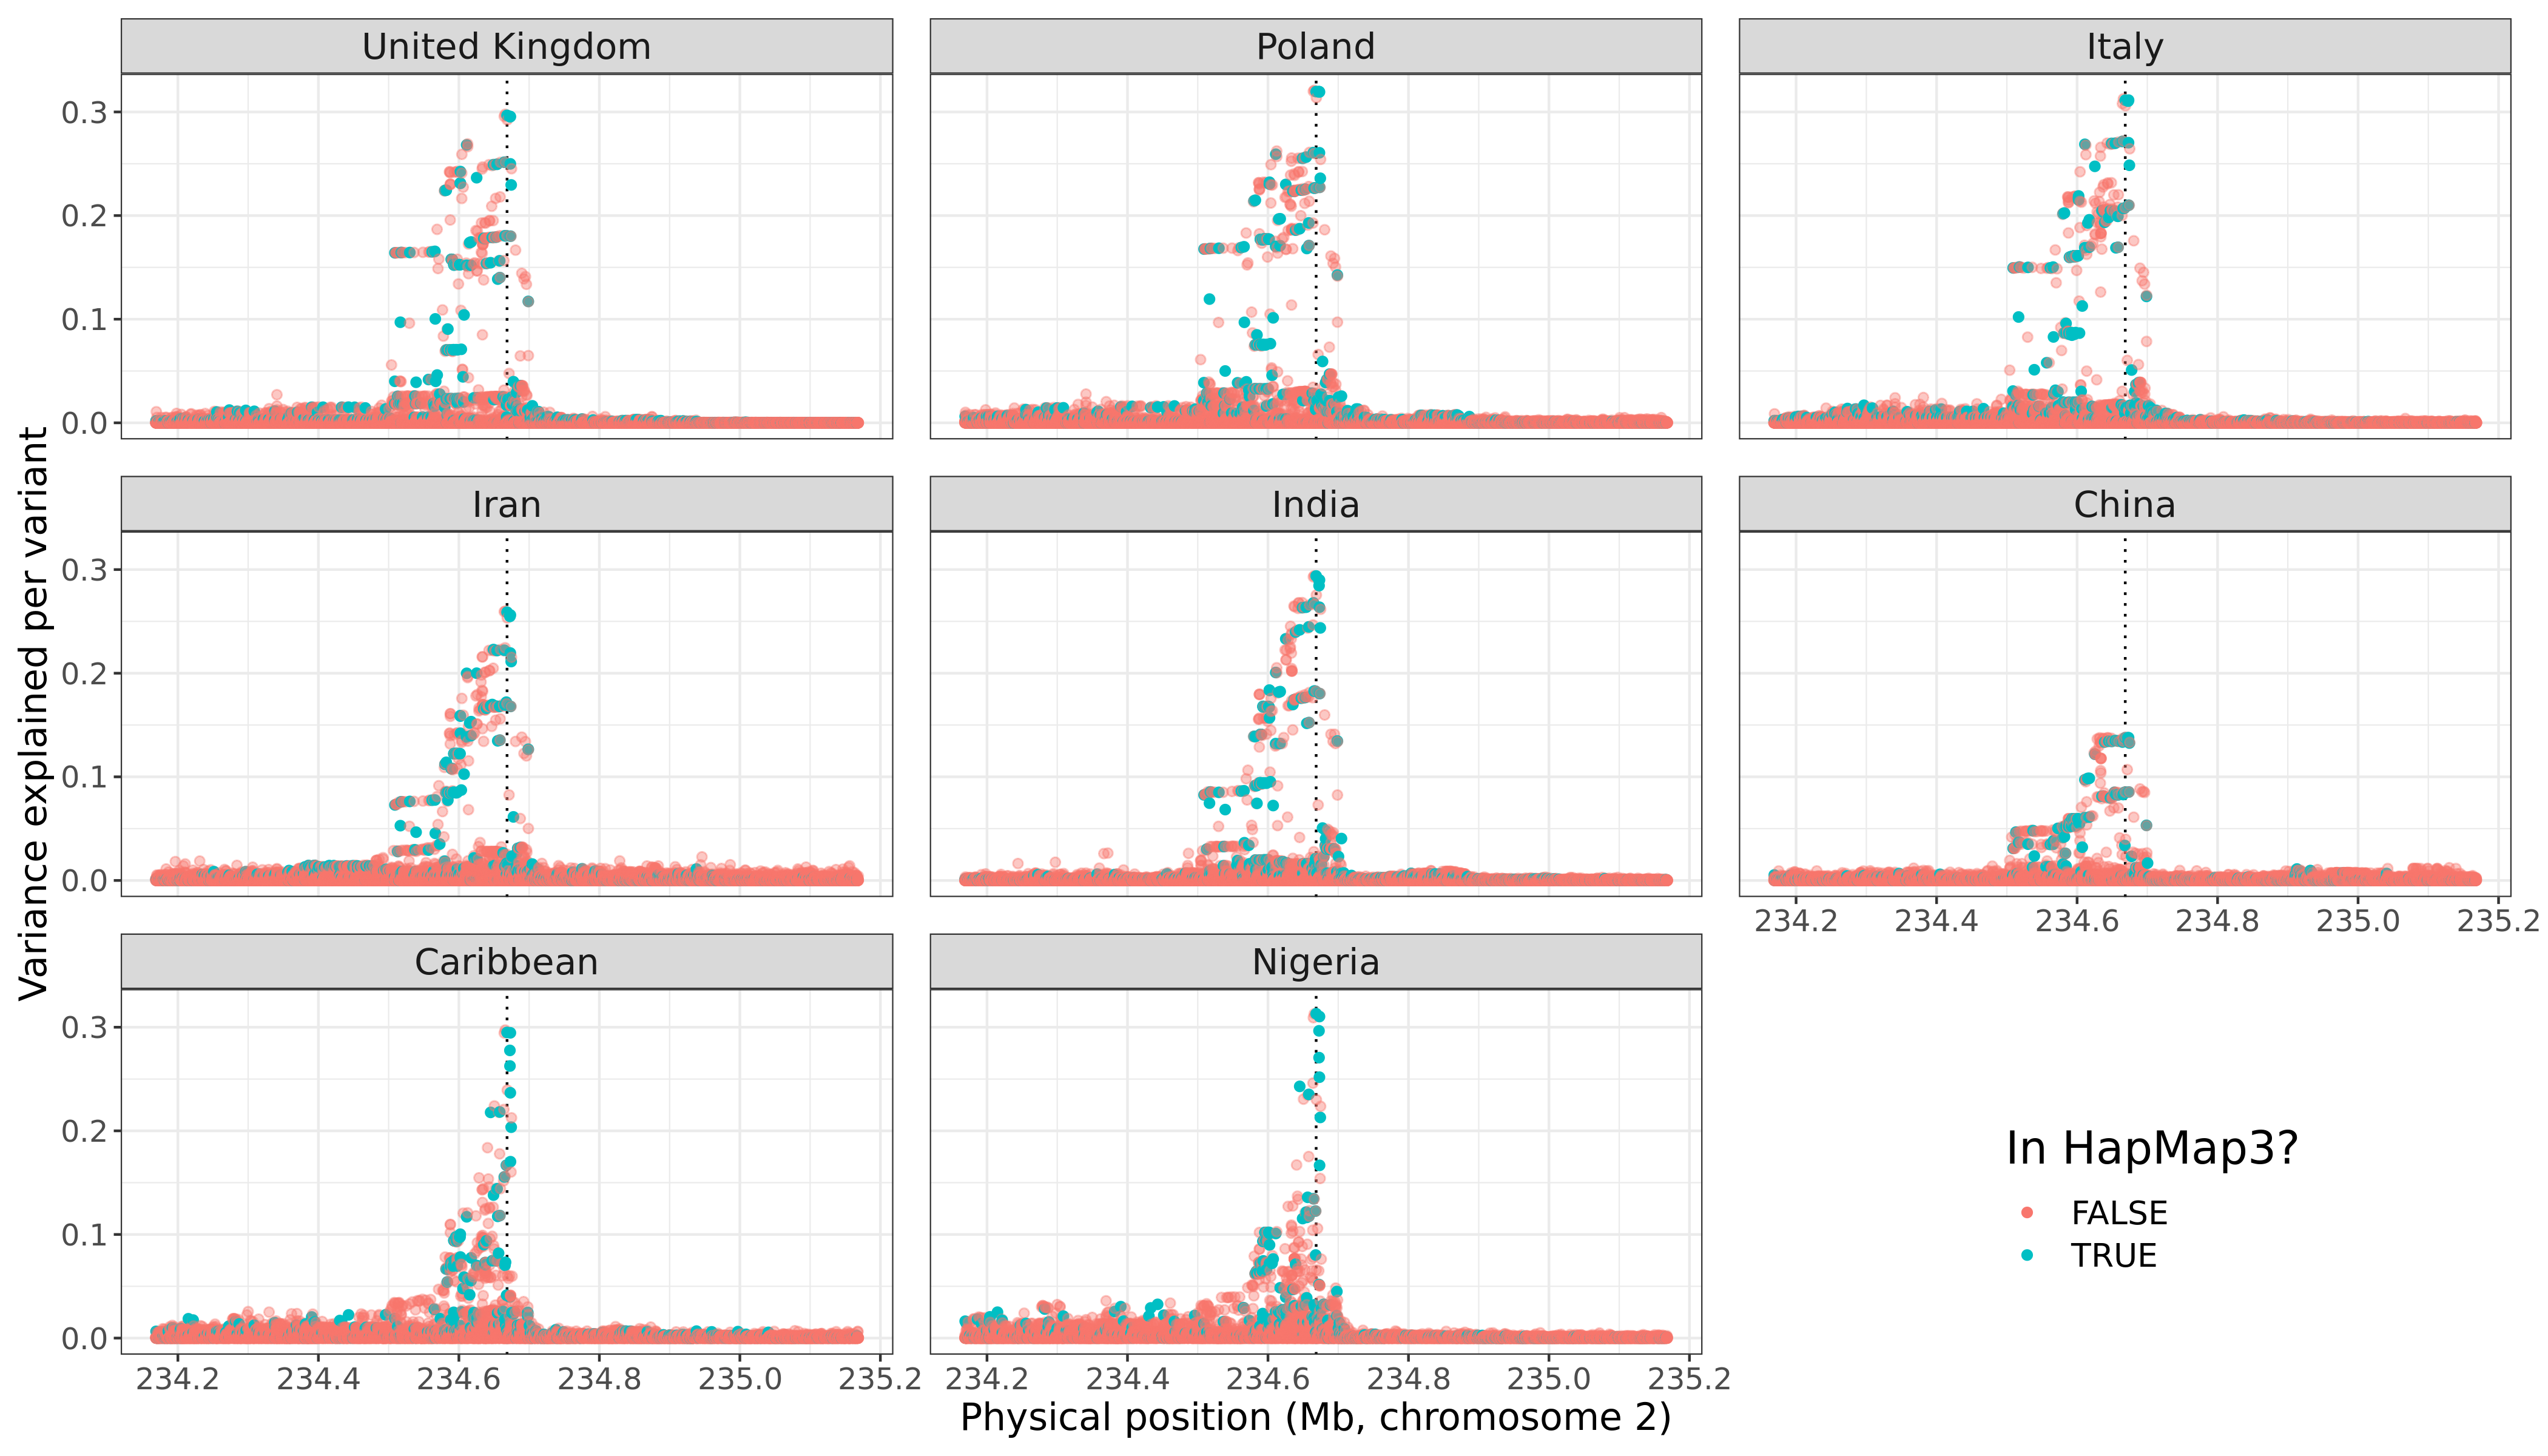
\includegraphics[width=0.9\textwidth]{zoom_log_bilirubin}
	\caption{Zoomed Manhattan plot for total \textbf{bilirubin} concentration. Here the (partial) correlation $r$ between each variant and the phenotype is reported, where $r = t / \sqrt{n + t^2}$, where $t$ is the t-score and $n$ is the degrees of freedom (the sample size minus the number of variables in the model, i.e.\ the covariates used in the GWAS, the intercept and the variant).The GWAS includes all variants with an imputation INFO score larger than 0.3 and within a 500Kb radius around the top hit from the GWAS performed in the UK training set and on the HapMap3 variants, represented by a vertical dotted line.}
	\label{fig:zoom-bilirubin}
\end{figure}

\begin{figure}[h]
	\centering
	\includegraphics[width=0.9\textwidth]{top3_log_bilirubin}
	\caption{Effect sizes and variance explained for the top three variants from figure \ref{fig:zoom-bilirubin}.}
	\label{fig:top3-bilirubin}
\end{figure}

\begin{figure}[h]
	\centering
	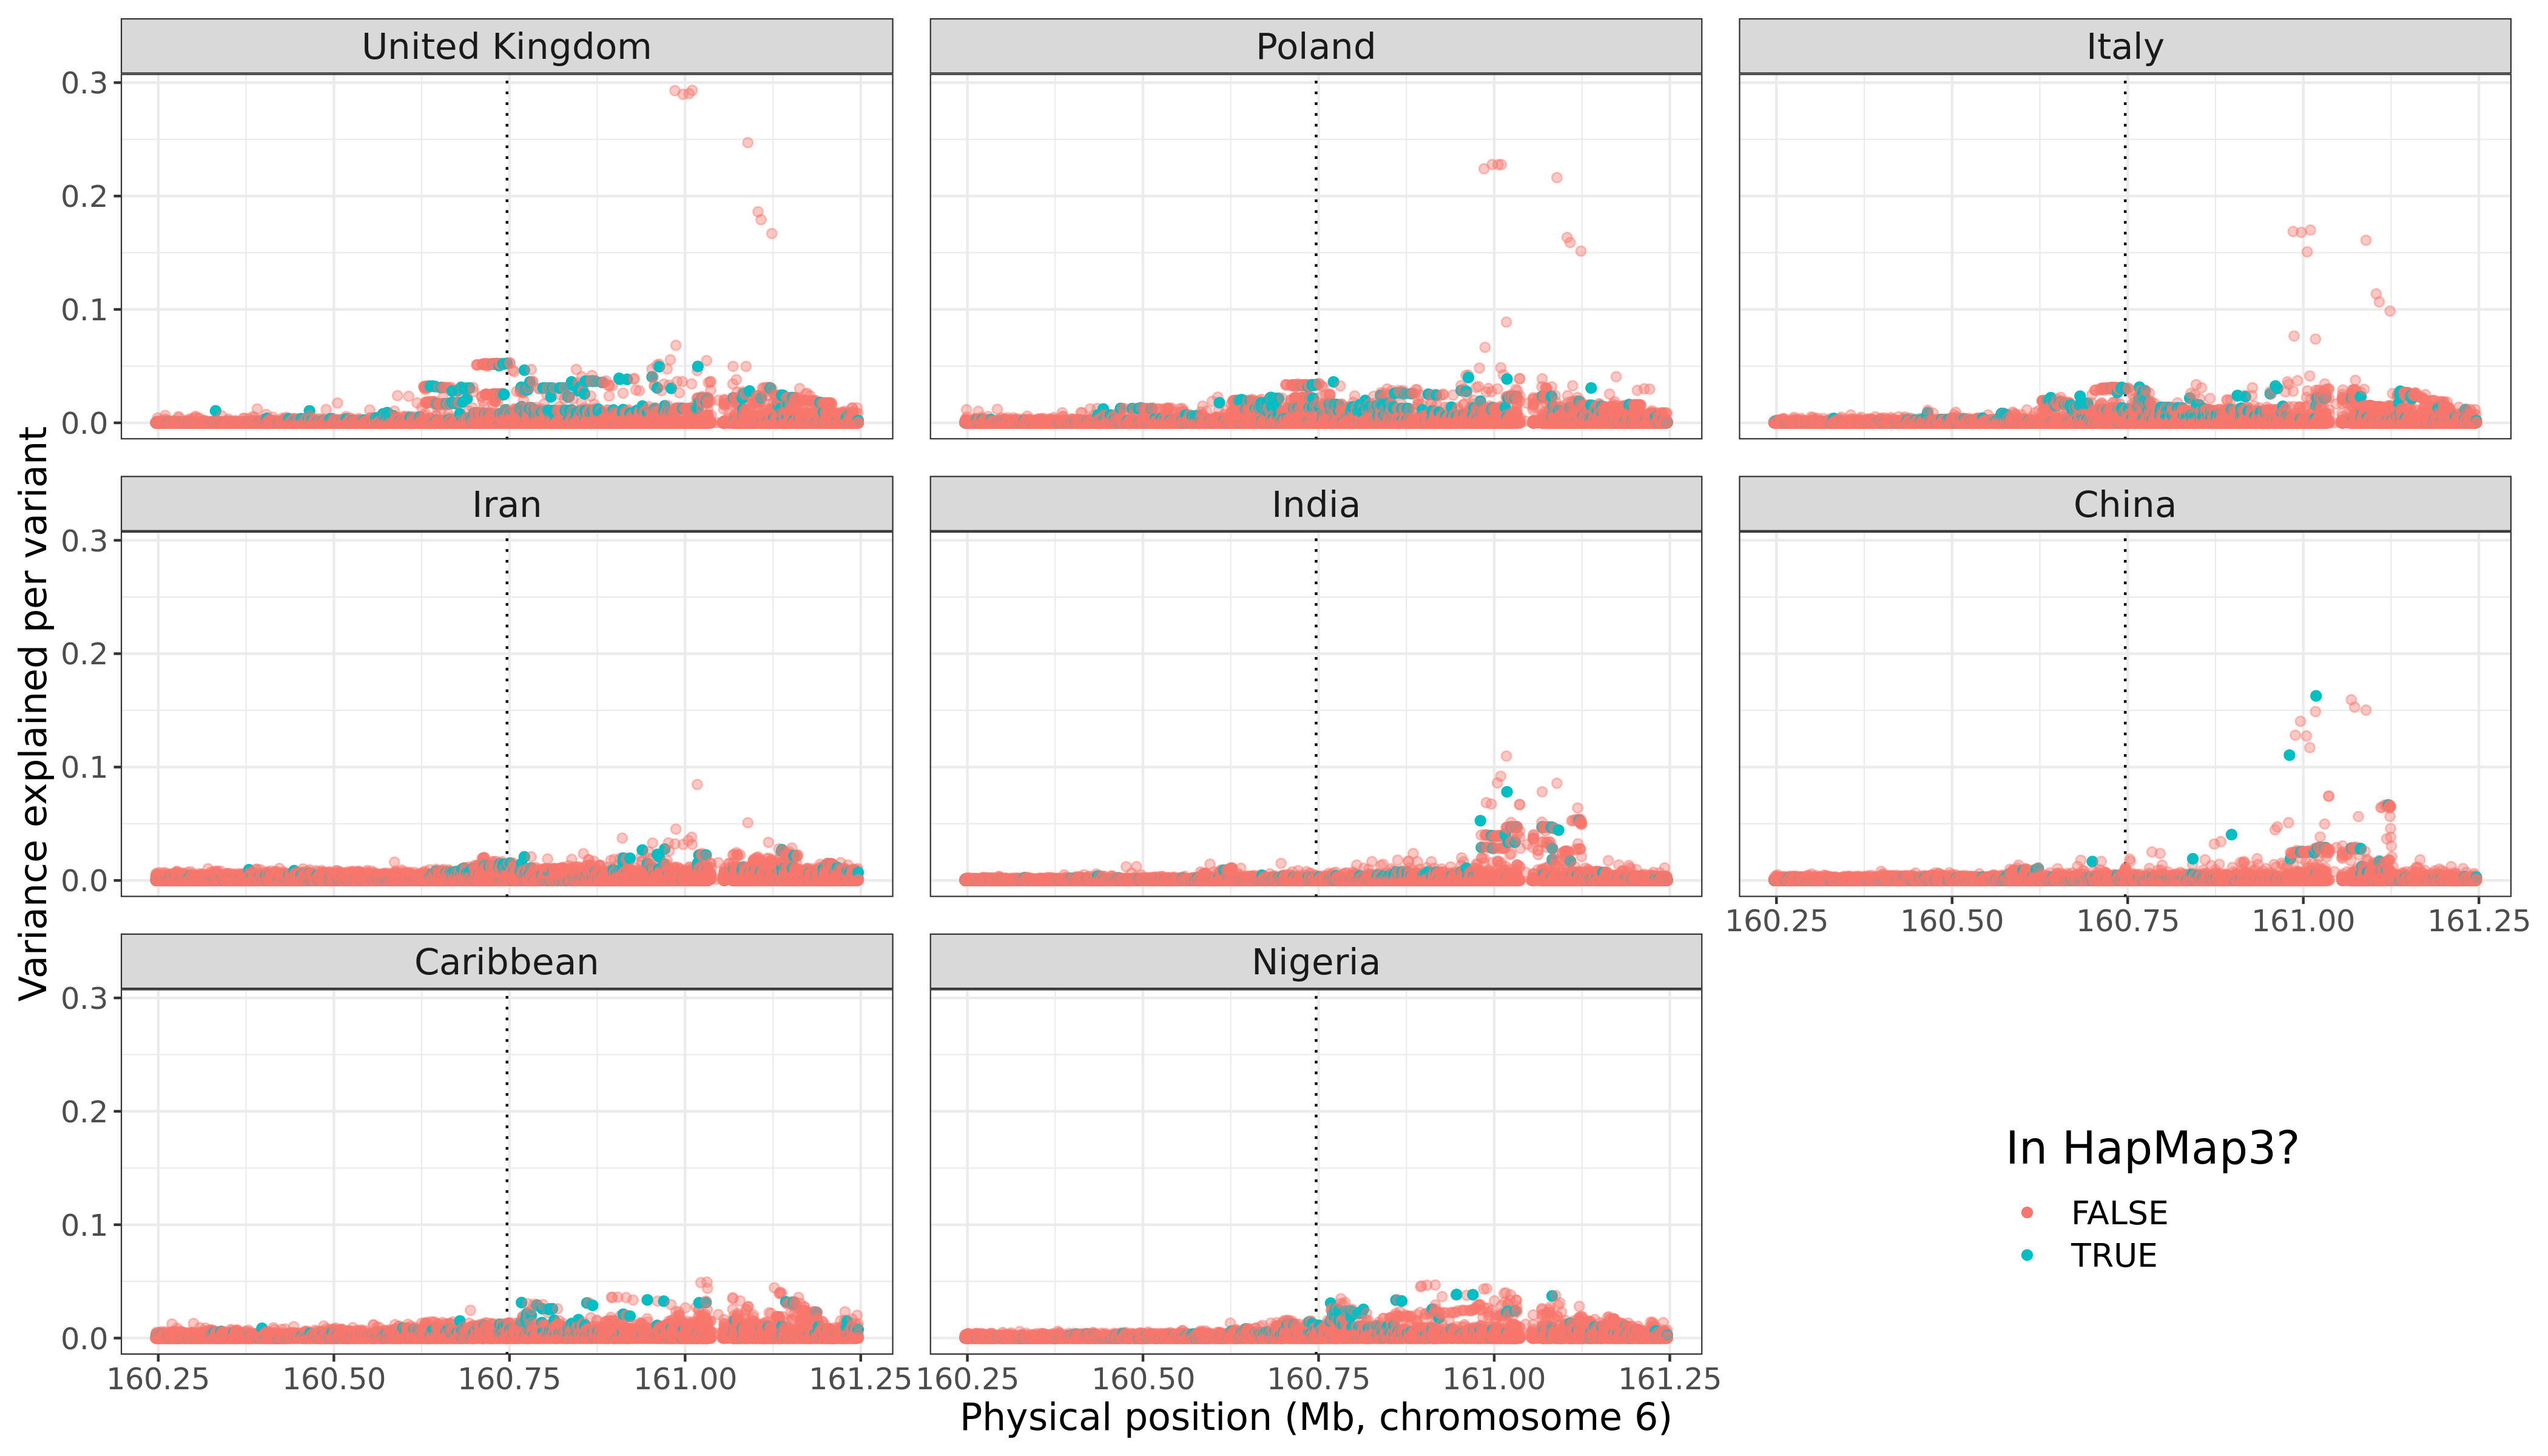
\includegraphics[width=0.9\textwidth]{zoom_log_lipoA}
	\caption{Zoomed Manhattan plot for \textbf{lipoprotein A} concentration. Here the (partial) correlation $r$ between each variant and the phenotype is reported, where $r = t / \sqrt{n + t^2}$, where $t$ is the t-score and $n$ is the degrees of freedom (the sample size minus the number of variables in the model, i.e.\ the covariates used in the GWAS, the intercept and the variant). The GWAS includes all variants with an imputation INFO score larger than 0.3 and within a 500Kb radius around the top hit from the GWAS performed in the UK training set and on the HapMap3 variants, represented by a vertical dotted line.}
	\label{fig:zoom-lipoA}
\end{figure}

\begin{figure}[h]
	\centering
	\includegraphics[width=0.9\textwidth]{top3_log_lipoA}
	\caption{Effect sizes and variance explained for the top three variants from figure \ref{fig:zoom-lipoA}.}
	\label{fig:top3-lipoA}
\end{figure}

\begin{figure}[h]
	\centering
	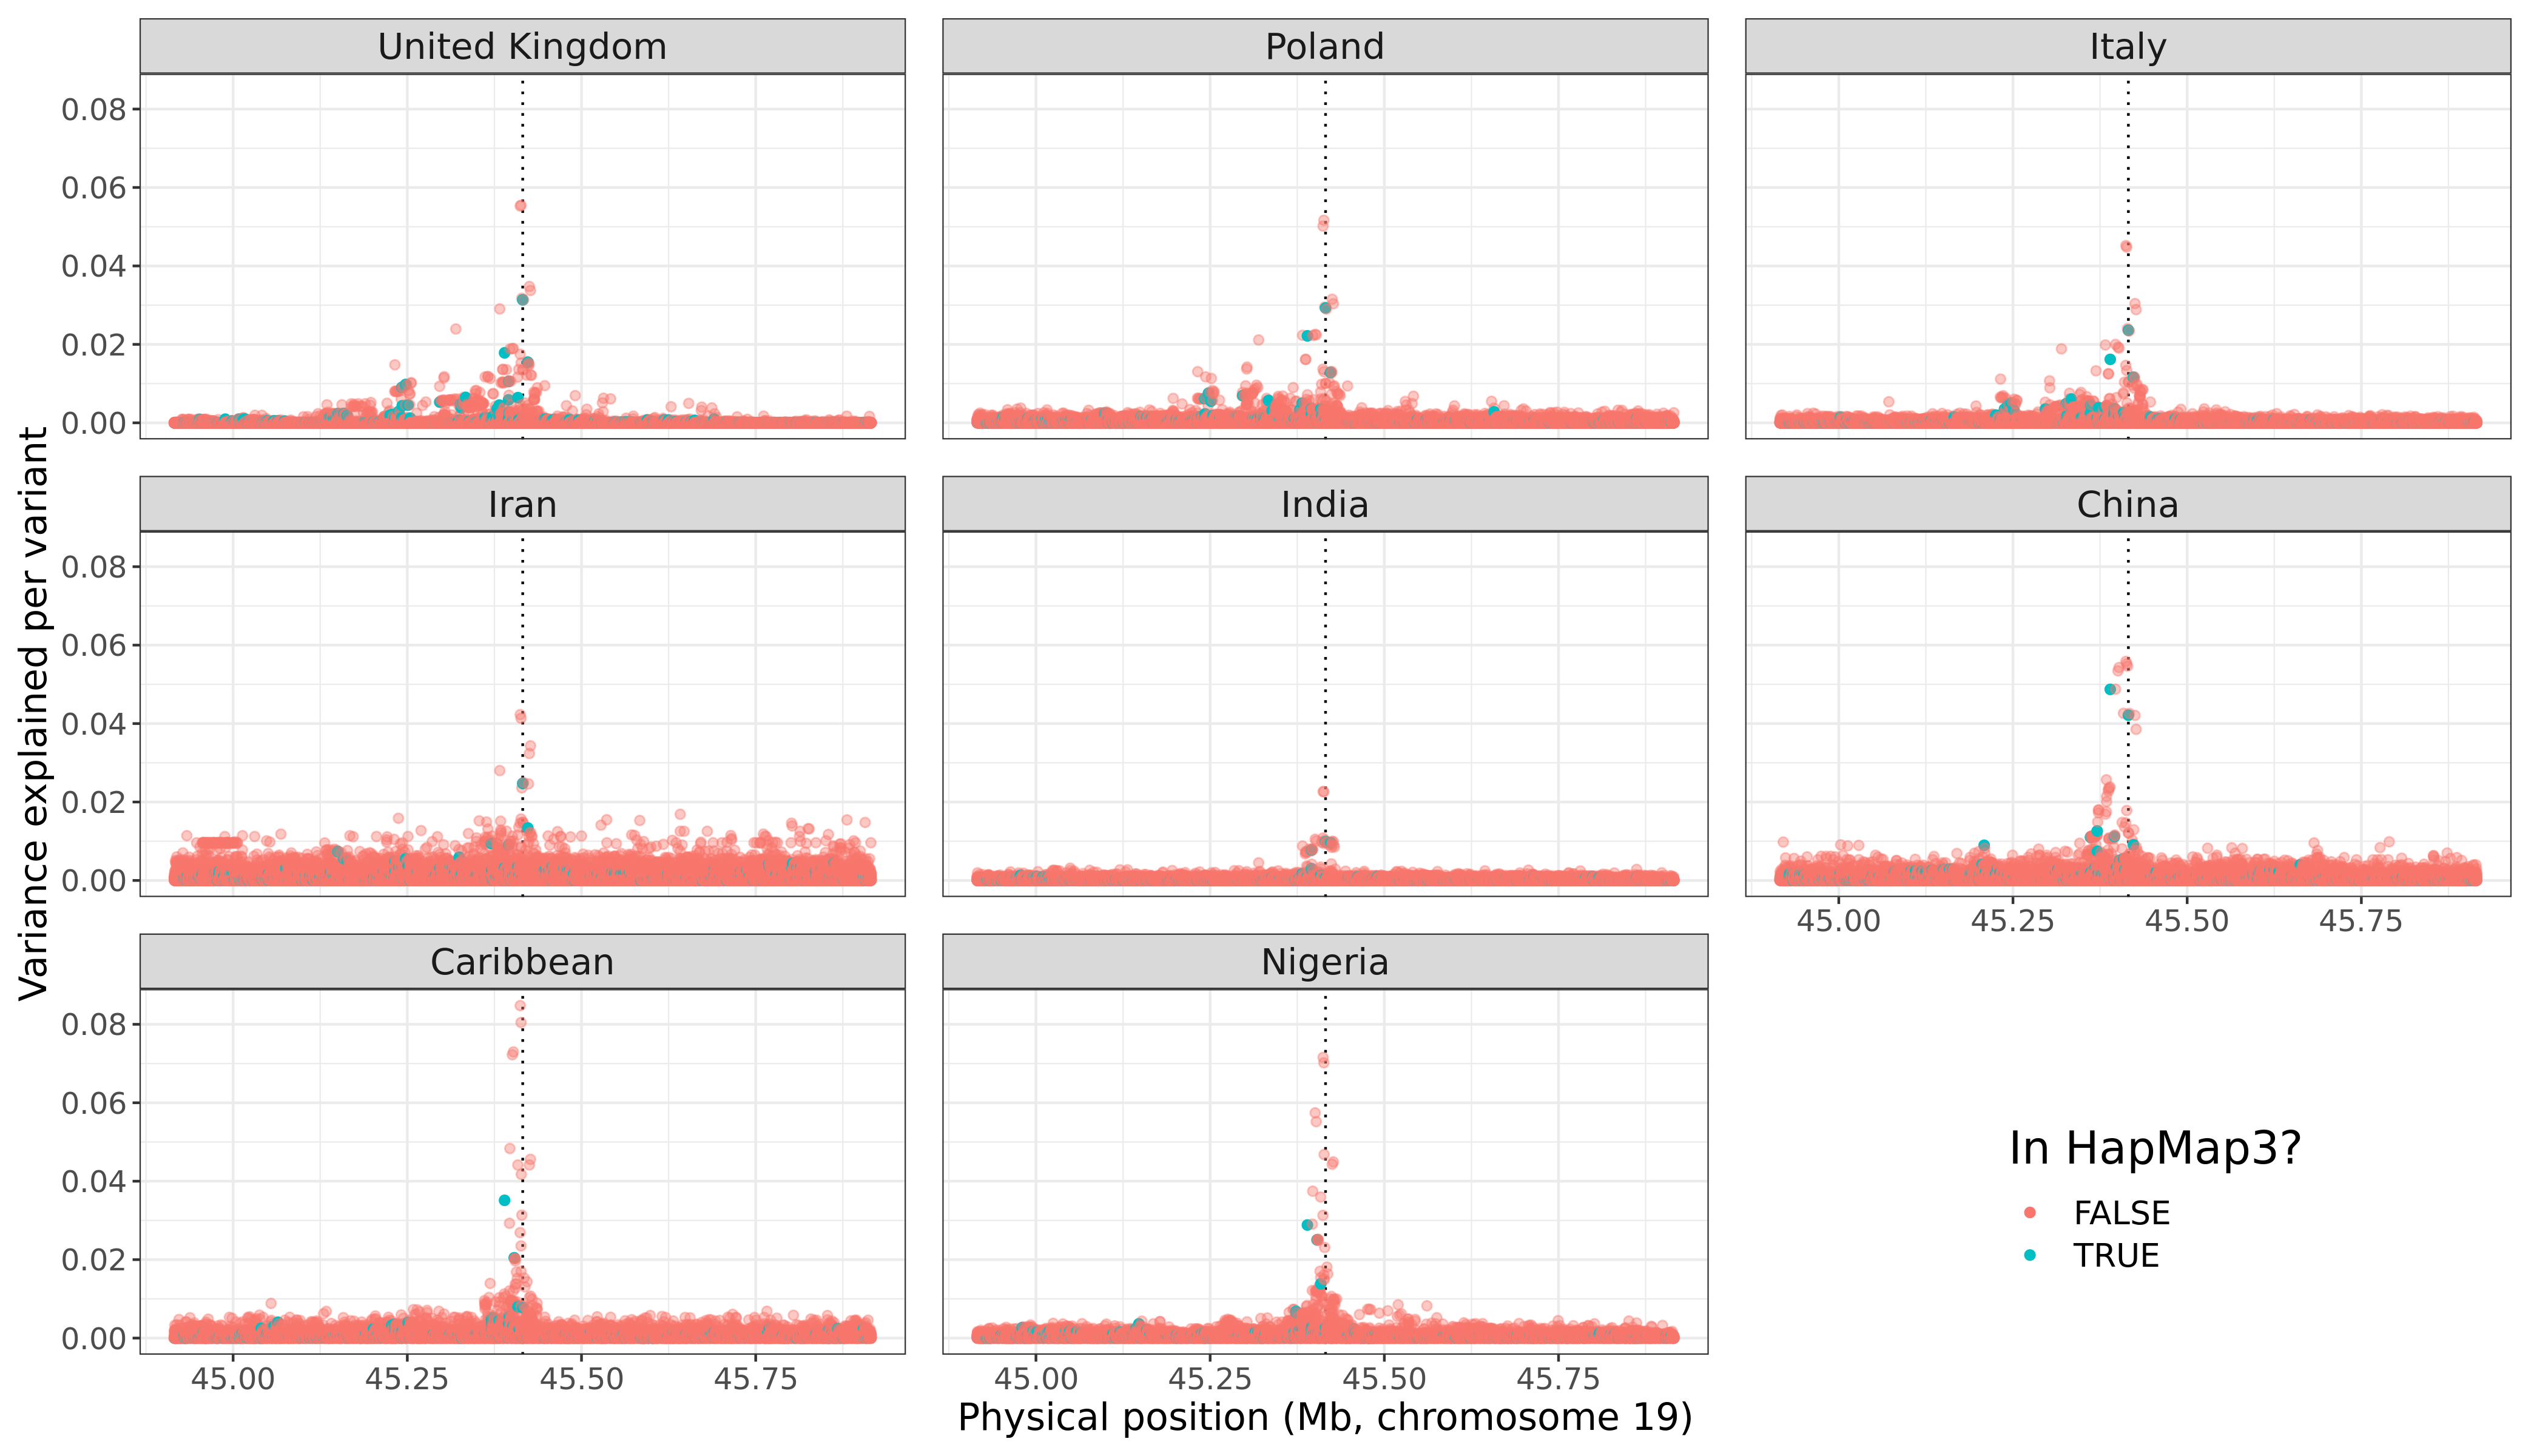
\includegraphics[width=0.9\textwidth]{zoom_apoB}
	\caption{Zoomed Manhattan plot for \textbf{apolipoprotein B} concentration. Here the (partial) correlation $r$ between each variant and the phenotype is reported, where $r = t / \sqrt{n + t^2}$, where $t$ is the t-score and $n$ is the degrees of freedom (the sample size minus the number of variables in the model, i.e.\ the covariates used in the GWAS, the intercept and the variant). The GWAS includes all variants with an imputation INFO score larger than 0.3 and within a 500Kb radius around the top hit from the GWAS performed in the UK training set and on the HapMap3 variants, represented by a vertical dotted line.}
	\label{fig:zoom-apoB}
\end{figure}

\begin{figure}[h]
	\centering
	\includegraphics[width=0.9\textwidth]{top3_apoB}
	\caption{Effect sizes and variance explained for the top three variants from figure \ref{fig:zoom-apoB}.}
	\label{fig:top3-apoB}
\end{figure}

%%%%%%%%%%%%%%%%%%%%%%%%%%%%%%%%%%%%%%%%%%%%%%%%%%%%%%%%%%%%%%%%%%%%%%%%%%%%%%%%

\begin{figure}[h]
	\centering
	\includegraphics[width=0.9\textwidth]{lasso_multi_pcor}
	\caption{Partial correlation achieved per phenotype (facets) and per ancestry group (x-axis) when training penalized regressions either with UK individuals only (training 1 in table 1) or when using individuals of multiple ancestries (training 2).}
	\label{fig:lasso-multi}
\end{figure}

%%%%%%%%%%%%%%%%%%%%%%%%%%%%%%%%%%%%%%%%%%%%%%%%%%%%%%%%%%%%%%%%%%%%%%%%%%%%%%%%

\begin{figure}[h]
	\centering
	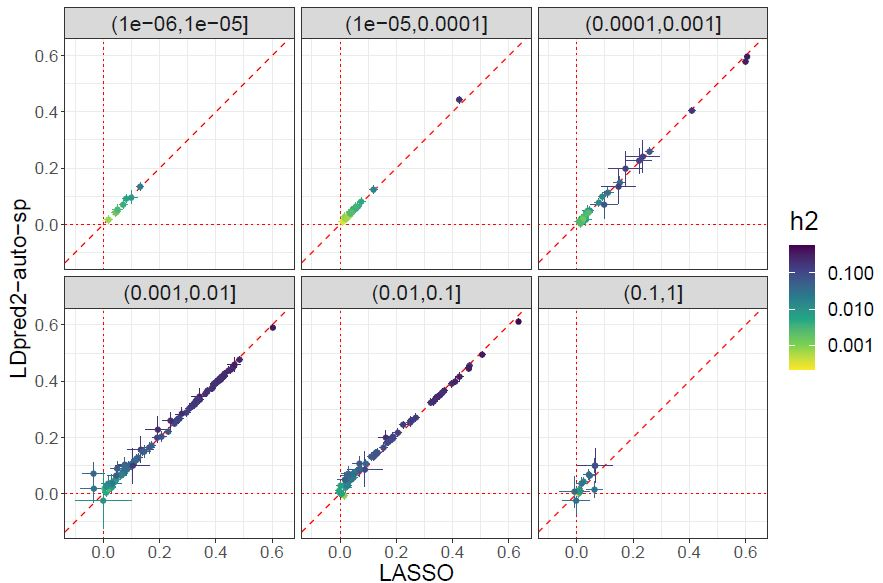
\includegraphics[width=0.9\textwidth]{PLR-ldpred2}
	\caption{\textbf{A)} Partial correlations (and 95\% CI) achieved per phenotype (each point) and per ancestry group (each facet) when training either with LASSO or with LDpred2-auto. \textbf{B)} Focus on the UK facet in A), facetting per proportion of causal variants $p$ and coloring by SNP heritability $h^2$ (estimates from LDpred2-auto).}
	\label{fig:plr-ldpred2}
\end{figure}

\begin{figure}[h]
\centering
\includegraphics[width=0.9\textwidth]{sparse-ldpred2}
\caption{Partial correlations achieved per phenotype (each point) and per ancestry group (each facet) when training either with LDpred2-auto or with LDpred2-auto-sparse (sparse option enabled).}
\label{fig:sparse-ldpred2}
\end{figure}

\begin{figure}[h]
	\centering
	\includegraphics[width=0.8\textwidth]{sparsity-plr}
	\caption{Proportion of variants with non-zero effects in the penalized regression models for each phenotype (point) versus the proportion of causal variants $p$ estimated from LDpred2-auto, colored by the partial correlation achieved in the UK test set.}
	\label{fig:sparsity-plr}
\end{figure}

\begin{figure}[h]
	\centering
	\includegraphics[width=0.8\textwidth]{sparsity-ldpred2}
	\caption{Proportion of variants with non-zero effects in LDpred2-auto-sparse for each phenotype (point) versus the proportion of causal variants $p$ estimated from LDpred2-auto, colored by the SNP heritability $h^2$ estimated from LDpred2-auto.}
	\label{fig:sparsity-ldpred2}
\end{figure}

%%%%%%%%%%%%%%%%%%%%%%%%%%%%%%%%%%%%%%%%%%%%%%%%%%%%%%%%%%%%%%%%%%%%%%%%%%%%%%%%

\begin{figure}[h]
	\centering
	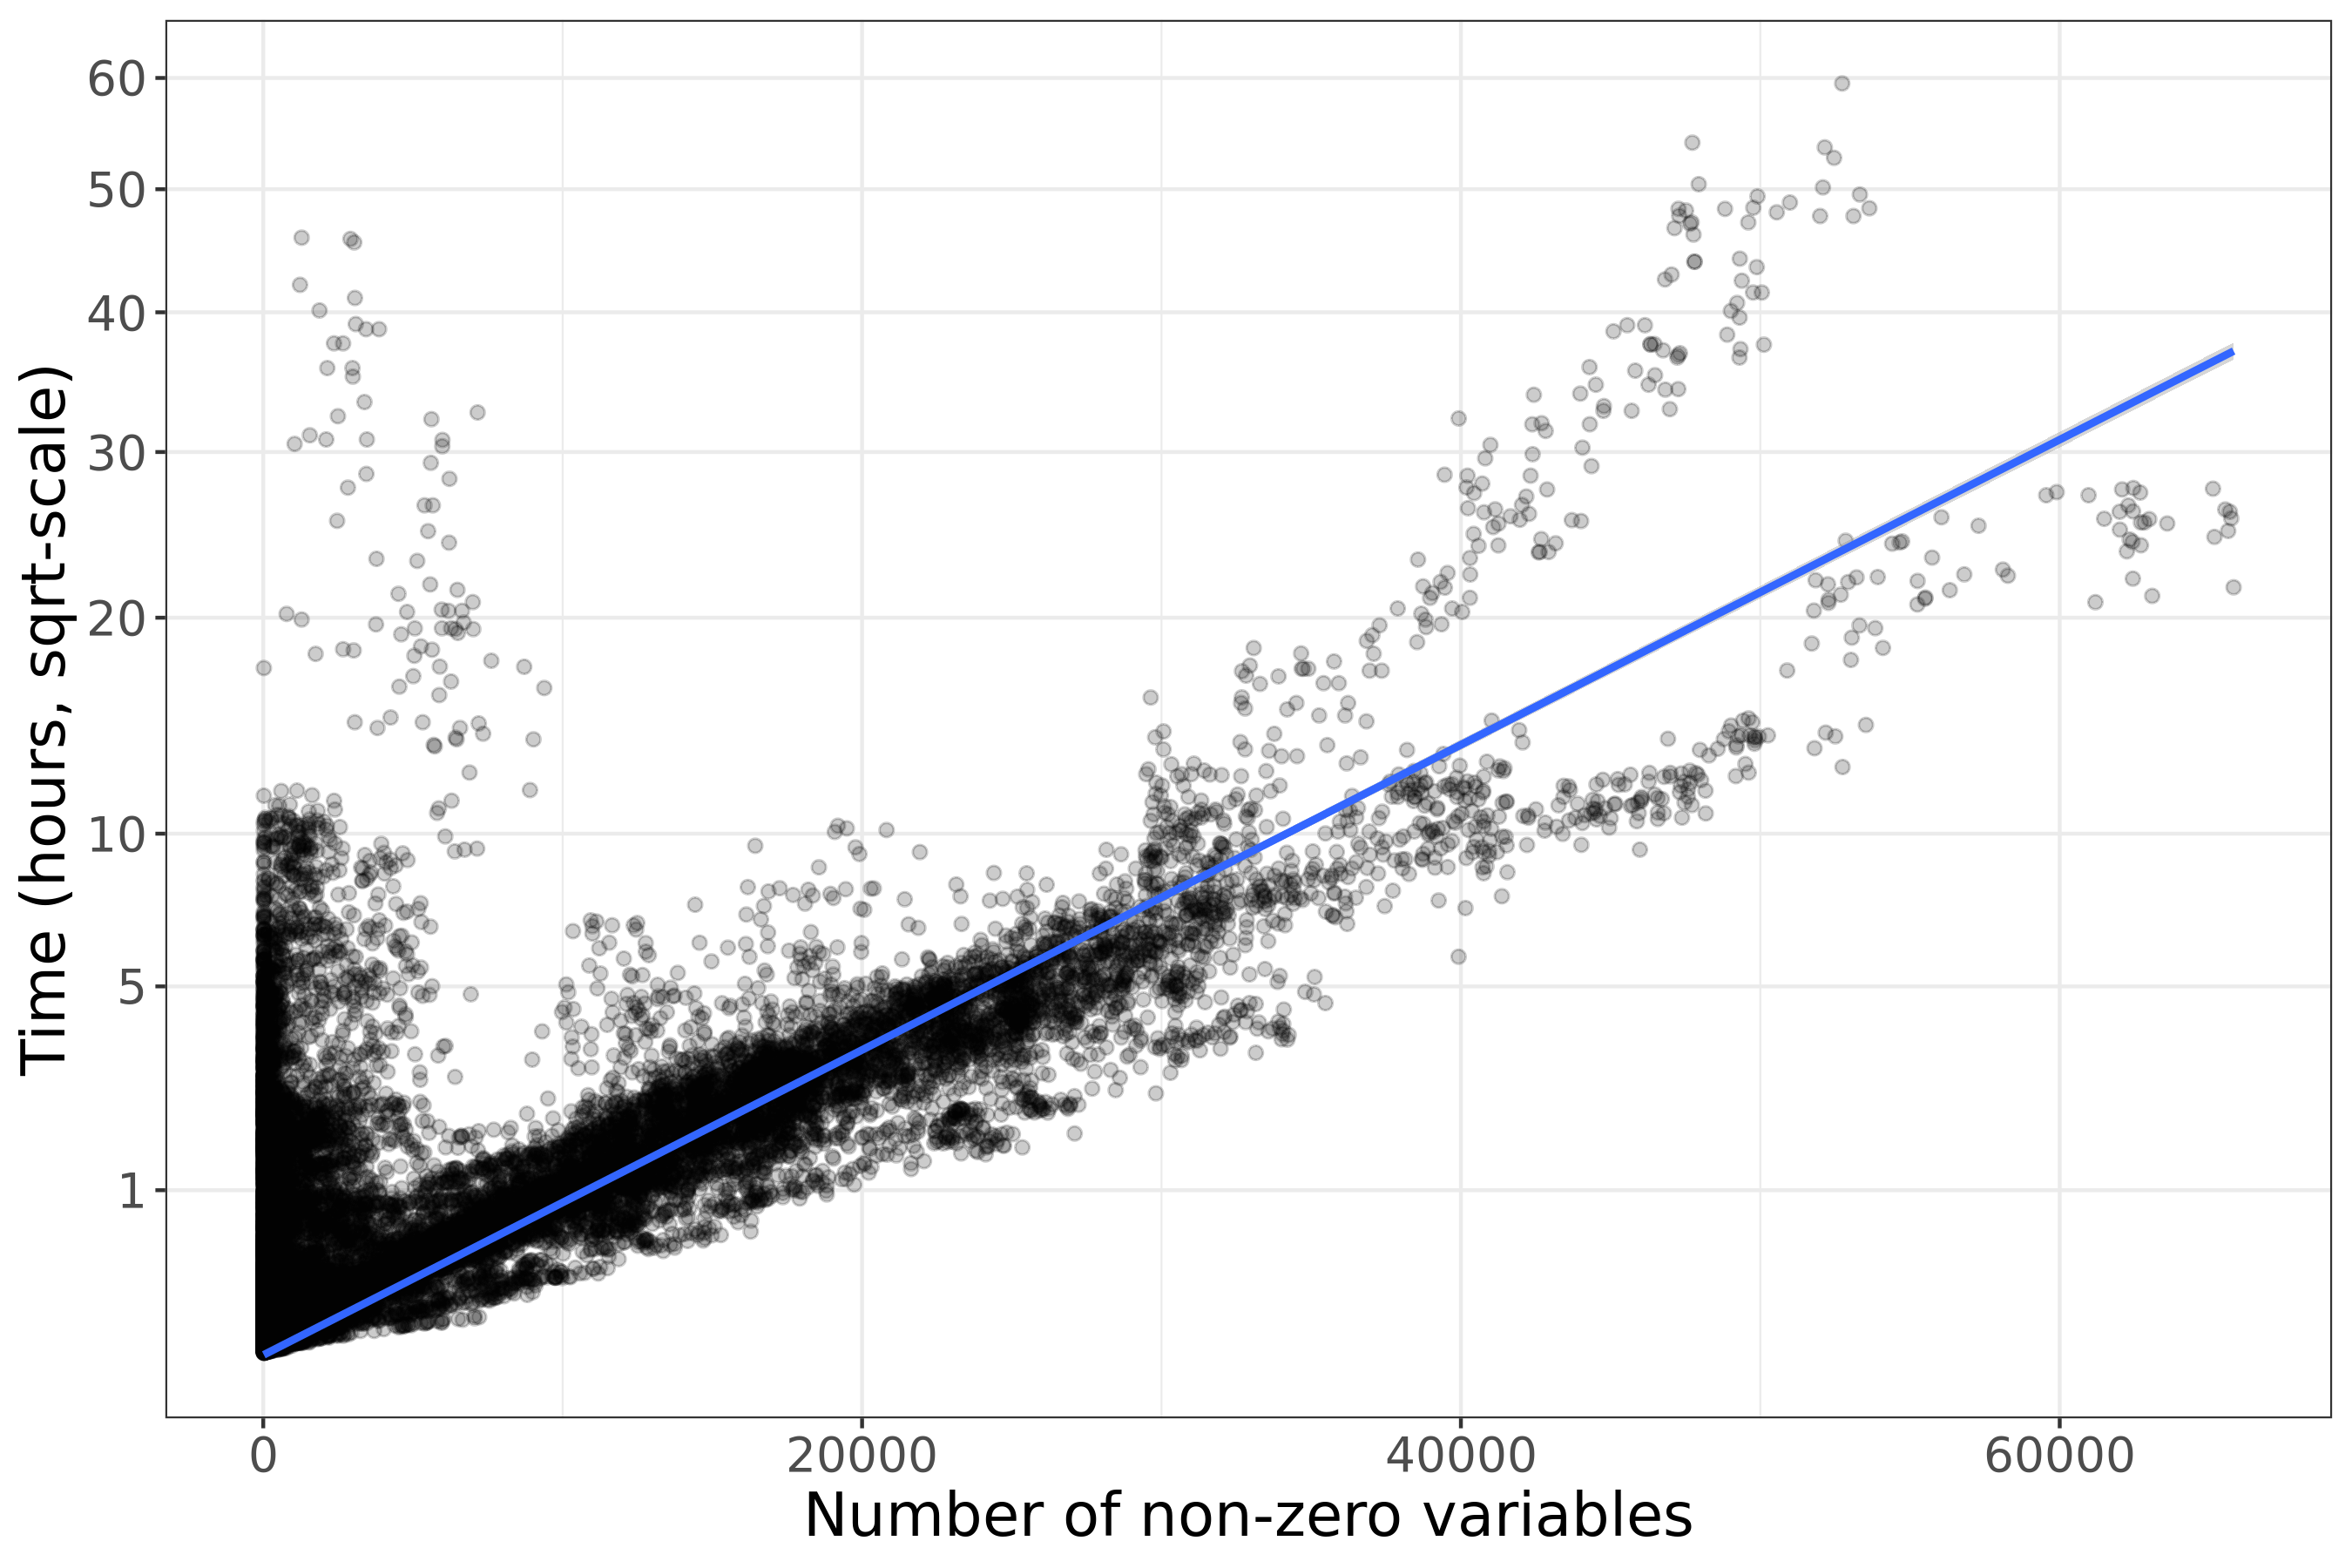
\includegraphics[width=0.9\textwidth]{timings}
	\caption{Computation times for all penalized regression models run using the 1M HapMap3 variants. We recall that we usually run 90 models for each phenotype because we use 9 sets of hyper-parameters and K=10 folds. Computation time is largely quadratic with the number of non-zero effects in the model. It is also dependent on the compute node and the loading of the HPC cluster at the time of running (Figure \ref{fig:timings-ldpred2}).}
	\label{fig:timings-plr}
\end{figure}

\begin{figure}[h]
	\centering
	\includegraphics[width=0.9\textwidth]{timings-ldpred2}
	\caption{Computation times for fitting LDpred2-auto (with default 1000 burn-in iterations + 500 more + sparse option running 150 more) using the 1M HapMap3 variants. Running times should be the same for all phenotypes, yet we see some variability depending on the node used. Some fitting had to be run again because it exceeded the 12-hour timeout, which happened a few times when and the HPC cluster was particularly crowded.}
	\label{fig:timings-ldpred2}
\end{figure}

%%%%%%%%%%%%%%%%%%%%%%%%%%%%%%%%%%%%%%%%%%%%%%%%%%%%%%%%%%%%%%%%%%%%%%%%%%%%%%%%

\begin{figure}[h]
	\centering
	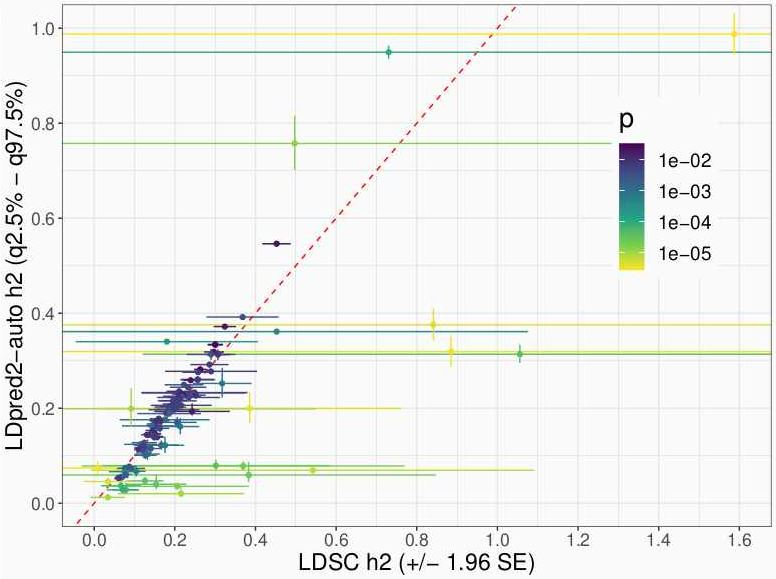
\includegraphics[width=0.9\textwidth]{heritability}
	\caption{SNP heritability $h^2$ estimates from LDpred2-auto versus LD score regression (using a 3cM window), for each phenotype (point) and colored by the proportion of causal variants $p$ estimated from LDpred2-auto. Heritability estimates for binary traits have been transformed to the liability scale (see Methods).}
	\label{fig:heritability}
\end{figure}

\begin{figure}[h]
\centering
\includegraphics[width=0.9\textwidth]{ldpred2-heritability-quant}
\caption{SNP heritability $h^2$ estimates from LDpred2-auto for continuous phenotypes, colored by the proportion of causal variants $p$ estimated from LDpred2-auto. }
\label{fig:heritability-quant}
\end{figure}

\begin{figure}[h]
\centering
\includegraphics[width=0.9\textwidth]{ldpred2-heritability-binary}
\caption{SNP heritability $h^2$ estimates from LDpred2-auto for binary phenotypes, colored by the proportion of causal variants $p$ estimated from LDpred2-auto.
Heritability estimates have been transformed to the liability scale (see Methods).}
\label{fig:heritability-binary}
\end{figure}

\begin{figure}[h]
	\centering
	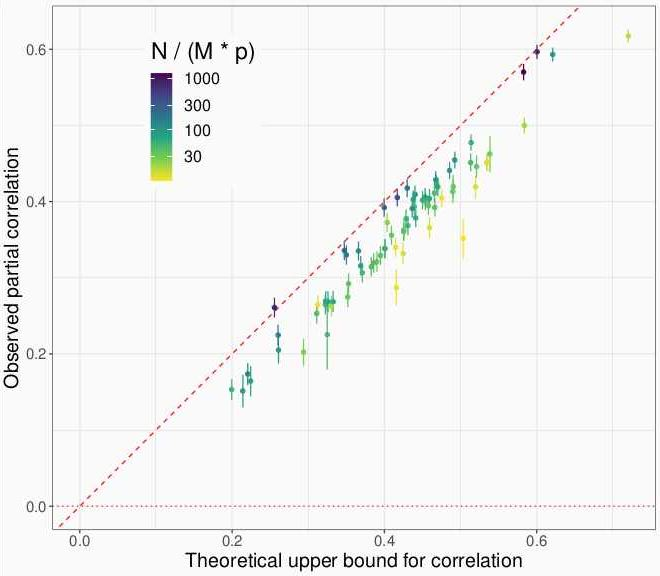
\includegraphics[width=0.9\textwidth]{upper-formula}
	\caption{Comparison between the observed partial correlation and the theoretical solution $r$ from the formula for the upper bound of the predictive accuracy of polygenic scores: $r^2 = \dfrac{h^2}{1 + (1 - r^2) \frac{M_c}{N h^2}}$, where $M_c = M \cdot p$ here.}
	\label{fig:upper-formula}
\end{figure}

\begin{figure}[h]
	\centering
	\includegraphics[width=0.9\textwidth]{power-pred-formula}
	\caption{Mean square error between the two axes in \ref{fig:upper-formula} when using $M_c = M \cdot p^\text{power}$. Minimum is obtained for $\text{power} = 0.68$.}
	\label{fig:power-pred-formula}
\end{figure}

\begin{figure}[h]
	\centering
	\includegraphics[width=0.9\textwidth]{pred-formula}
	\caption{Same as figure \ref{fig:upper-formula} when using $M_c = M \cdot p^{0.68}$, where 0.68 is the argmin in figure \ref{fig:power-pred-formula}.}
	\label{fig:pred-formula}
\end{figure}

%%%%%%%%%%%%%%%%%%%%%%%%%%%%%%%%%%%%%%%%%%%%%%%%%%%%%%%%%%%%%%%%%%%%%%%%%%%%%%%%

\begin{figure}[htbp]
	\centerline{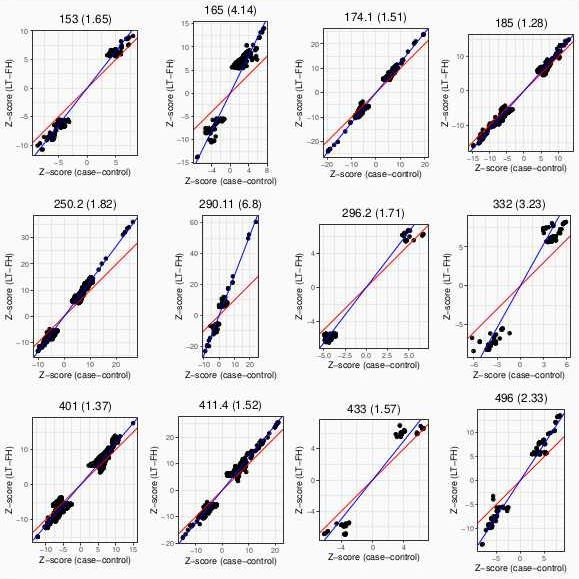
\includegraphics[width=0.95\textwidth]{power_LTFH}}
	\caption{Z-Scores from GWAS using case-control phenotypes and LT-FH phenotypes. Only genome-wide significant variants are represented. The slope (in blue) is computed using Deming regression using the inverse of the absolute value as standard deviations (to put more weight on the more significant variants).
	In the title are reported the phecode as well as this slope (squared), which we report as the power multiplier.}
	\label{fig:power-ltfh}
\end{figure}

\begin{figure}[htbp]
\begin{subfigure}{\textwidth}
\centering
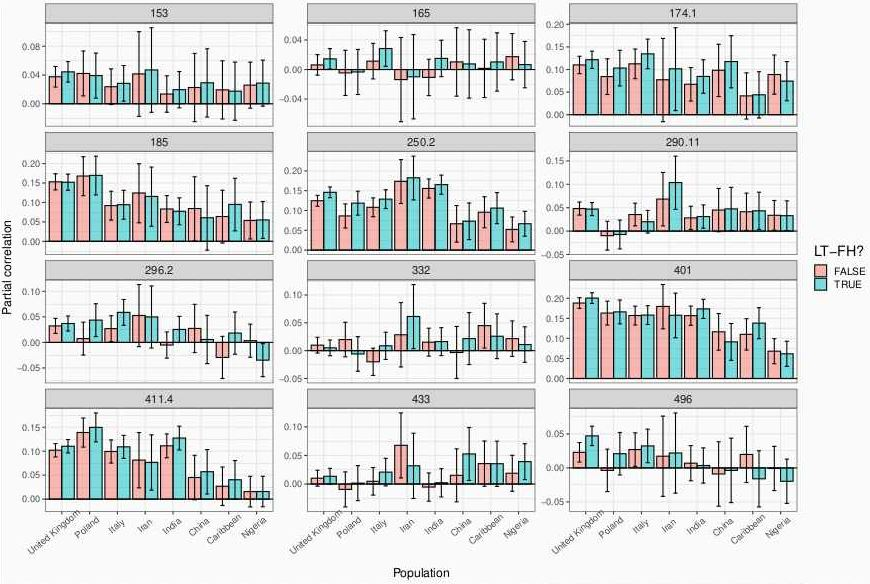
\includegraphics[width=.85\linewidth]{lasso_LTFH}
\end{subfigure}\vspace{1em}
\begin{subfigure}{\textwidth}
\centering
\includegraphics[width=.85\linewidth]{lasso_LTFH2}
\end{subfigure}
\caption{Two subfigures presenting the same results, the partial correlation achieved per phenotype and per population when using either the normal case-control phenotype for training or the phenotype derived using LT-FH. Partial correlations are always derived using the case-control phenotypes in the test set.}
\label{fig:lasso-ltfh}
\end{figure}

%%%%%%%%%%%%%%%%%%%%%%%%%%%%%%%%%%%%%%%%%%%%%%%%%%%%%%%%%%%%%%%%%%%%%%%%%%%%%%%%

\begin{figure}[htbp]
	\centerline{\includegraphics[width=0.9\textwidth]{qc-plot-new-formula}}
	\caption{Comparison of the standard deviations (SD) computed from both genotypes and summary statistics for the 1000 most associated variants with bilirubin concentration. A) uses the previous formula $\text{sd}(\boldsymbol{G_j}) \approx \frac{\text{sd}(\boldsymbol{y})}{\sqrt{n ~ \text{se}(\hat{\gamma}_j)^2}}$ proposed in \cite{prive2020ldpred2} while B) uses the updated formula $\text{sd}(\boldsymbol{G_j}) \approx \frac{\text{sd}(\boldsymbol{y})}{\sqrt{n ~ \text{se}(\hat{\gamma}_j)^2 + \hat{\gamma}_j^2}}$ proposed here, which does one less approximation.
	The slope slightly larger than 1 can be explained by $\text{sd}(\boldsymbol{y}) > \text{sd}(\boldsymbol{\breve{y}})$.}
	\label{fig:new-formula}
\end{figure}

%%%%%%%%%%%%%%%%%%%%%%%%%%%%%%%%%%%%%%%%%%%%%%%%%%%%%%%%%%%%%%%%%%%%%%%%%%%%%%%%

\clearpage


%%%%%%%%%%%%%%%%%%%%%%%%%%%%%%%%%%%%%%%%%%%%%%%%%%%%%%%%%%%%%%%%%%%%%%%%%%%%%%%%

\clearpage

\bibliographystyle{natbib}
\bibliography{refs}

\end{document}
